\chapter{Statistical Hypothesis Testing} \label{ch:ht}

A statistical hypothesis test is a method of statistical inference used to decide whether the empirical data sufficiently support a particular hypothesis. Details are given in the rest of the chapter.

\section{Hypothesis}

This section illustrates the concept of hypothesis and the purpose of hypothesis testings.

\subsection{Motivating Examples}

Two motivating examples are considered.

\begin{shortbox}
\Boxhead{Example: Verify the Probability of a Coin Tossing ``Head''}

Consider tossing a coin. The result follows Bernoulli distribution with the chance of head $p$ and tail $1-p$. For a normally designed coin, it is fair to assume that $p=0.5$. Toss the coin multiple times. Consider the following events:
\begin{enumerate}
	\item Toss the coin 1 time and the result is ``head'';
	\item Toss the coin 5 times and all the results are ``head'';
	\item Toss the coin 10 times and all the results are ``head''.
\end{enumerate}

If the above events happen, how confident are we to insist that the coin tossing has a probability of head of $p=0.5$?

\end{shortbox}

If $p=0.5$ is indeed correct, the probabilities of the 3 events are $P=0.5$, $P=0.5^5=0.03125$ and $P=0.5^{10}= 0.0009765625$ respectively. These figures are consistent with our intuition: the first event can happen quite often, the second very rare, and third seemingly never happen in real life. On the other hand, if the third indeed happens in the first trail, then it is very likely that it is a specially designed coin and $p>0.5$.

To verify whether $p=0.5$ or $p>0.5$, we can make an hypothesis $H_0:p=0.5$ as well as its alternative hypothesis $H_1:p>0.5$ . The Bernoulli trail results then can be used to support or reject the hypothesis with quantified probability. Details are discussed in the remaining of this chapter. 

\begin{shortbox}
\Boxhead{Example: Interview People for Average Annual Income}

Consider another example of estimating the average monthly income of the population in a city. It is too costly to interview all the $n=1000000$ citizens in the city. Therefore, only $1\%$ of the population, $m=10000$ people, are randomly selected and interviewed.

The purpose is to evaluate whether the average income is at least $\$3,000$. 

\end{shortbox}

In this example, the hypothesis is $H_0: \bar{X} \geq 3000$ where $\bar{X}$ is the mean of income of the entire population. Its alternative hypothesis is $H_1: \bar{X}<3000$. The interview results obtained from the $m$ samples are used to support or reject the hypothesis.

Both the above two examples verify the aggregated mean of a parameter using hypothesis testings. It is possible to use hypothesis testing for other figures as well, including variance and many more. An example is given below. In the first coin tossing example, the coin manufacture has claimed that the probability of head $p$ follows a normal distribution of $\mathcal{N}(0.5,0.01^2)$. We can use hypothesis testing to verify whether $H_0:\sigma^2=0.01^2$ or $H_1:\sigma^2>0.01^2$.

\subsection{Hypothesis Categories}

The baseline hypothesis, such as ``$p=0.5$ to give head when tossing a coin'' in the motivating example, is known as the \mync{null hypothesis} which is often denoted by $H_0$. One way of interpreting ``null'' in this context is that it is the default ``boring'' hypothesis that nulls any changes or innovations. The alternative to the null hypothesis is known as the \mync{alternative hypothesis} which is often denoted by $H_1$ or $H_a$.

We take the null hypothesis as the ``default truth''. There is no need, or it is not possible, to directly prove that the null hypothesis is correct. So we look at a different approach to see whether we can prove it wrong, which is why hypothesis test is introduced. Hypothesis test focuses on looking for evidence to disprove the null hypothesis. The samples try to reject the null hypothesis and the hypothesis test checks whether there is strong evidence in the samples that allow them to do so.

When the samples fail to reject the null hypothesis, it does not necessarily mean that the samples support the hypothesis. It is just that there is no strong statistical evidence in the samples to disprove the hypothesis.

Depending on the statement made in the null hypothesis, it can be divided into two categories: \mync{simple hypothesis} where it specifies a particular precise value for each parameter, or \mync{compound hypothesis} where it specifies multiple values or ranges of values for at least one of the parameters. 

\subsection{Acceptance Region and Rejection Region}

A hypothesis is tested using the samples. Since the samples are randomly picked form the population, the result of a hypothesis test, could be random to some extent.

Let $X_1, \ldots, X_m$ be the $m$ samples taken in the trail. It may just so happen that this particular set of samples passes or fails the hypothesis test. Define
\begin{eqnarray}
	A &=& \left\{\left(x_1, \ldots, X_m\right)\middle| H_0 \textup{~is accepted}\right\} \label{eq:htest_a} \\
	R &=& \left\{\left(x_1, \ldots, X_m\right)\middle| H_0 \textup{~is rejected}\right\} \label{eq:htest_r}
\end{eqnarray}
as the \mync{acceptance region} and \mync{rejection region} respectively. Notice that the rejection region is also known as the \mync{critical region}. 

The probability of the null hypothesis being rejected relates to the cardinality of the acceptance and rejection regions. The \mync{power function} is used to describe the probability that the samples reject the null hypothesis $H_0$. The denotation is given below.
\begin{eqnarray}
	\beta_\Phi(\theta) &=& P\left(\left(\begin{array}{ccc}
		X_1, & \ldots, & X_m
	\end{array}\right)\in R\right) \nonumber
\end{eqnarray}
where $\theta$ is the true value of the parameter under testing, and $\Phi$ the hypothesis testing method.

When $\theta$ is such that $H_0$ is actually true, there is still a possibility that by unlucky sampling $H_0$ is rejected, and the probability is given by $\beta_\Phi(\theta)$. In that scenario, we would like $\beta_\Phi(\theta)$ to be small. On the contrary, when $\theta$ is such that $H_0$ is actually false, there is still a possibility that by unlucky sampling $H_0$ is accepted, and the probability is given by $1-\beta_\Phi(\theta)$. In that scenario, we would like $\beta_\Phi(\theta)$ to be large. The value of $\beta_\Phi(\theta)$ under these two scenarios can be used to evaluate the effectiveness of a hypothesis testing method.

Consider the case where $H_0$ is true. In this case, the power function describes the probability of the hypothesis test making a \mync{type I error}: reject a true null hypothesis. The probability is described by
\begin{eqnarray}
	\alpha_{1\Phi}(\theta) &=& \left\{\begin{array}{cc}
		\beta_\Phi(\theta) & H_0 \textup{~is true} \\
		0 & H_0 \textup{~is false}
	\end{array}\right. \label{eq:hypotestalpha1}
\end{eqnarray}
On the other hand, when $H_0$ is false, the power function describes (the compensation of) the probability of the hypothesis test making a \mync{type II error}: fail to reject a false null hypothesis. The probability is described by
\begin{eqnarray}
	\alpha_{2\Phi}(\theta) &=& \left\{\begin{array}{cc}
		0 & H_0 \textup{~is true} \\
		1-\beta_\Phi(\theta) & H_0 \textup{~is false}
	\end{array}\right. \label{eq:hypotestalpha2}
\end{eqnarray}

Ideally, a good hypothesis test shall ensure that both \eqref{eq:hypotestalpha1} and \eqref{eq:hypotestalpha2} are small. However, notice that there is a trade-off. An very small \eqref{eq:hypotestalpha1}, for example by acting extremely conservative and not rejecting any hypothesis regardless of the samples, may lead to a very large \eqref{eq:hypotestalpha2}, and vise versa. In a common practice, a \mync{significance level}, $\alpha$, is defined for \eqref{eq:hypotestalpha1}. The target to minimize \eqref{eq:hypotestalpha2} while keeping \eqref{eq:hypotestalpha1} equal or below $\alpha$. Typical values of $\alpha$ include $0.05$, $0.01$, etc. 

For two hypothesis testing methods $\Phi_1$ and $\Phi_2$ that both satisfy the same significance level, their $\alpha_{2\Phi}(\theta)$ decide which one is more reliable. The lower $\alpha_{2\Phi}(\theta)$, the better the quality of the hypothesis testing. Among all the hypothesis testing methods that satisfies the same significance level $\alpha$, if there is a hypothesis testing method $\Phi$ that gives the smallest $\alpha_{2\Phi}(\theta)$ in \eqref{eq:hypotestalpha2}, $\Phi$ is known as the uniformly optimal hypothesis testing method at significance level $\alpha$. Notice that it is challenging to find and prove the uniform optimal of a hypothesis testing method which usually requires a lot of statistics expertise.

\section{Commonly Seen Hypothesis Tests}

We have seen some hypothesis tests problems in the motivating examples. More are introduced in this section, together with their solutions.

\subsection{The Mean of a Normal Distribution}

Let parameter $\theta$ follow normal distribution $\mathcal{N}(\mu,\sigma^2)$, where $\sigma^2$ might be unknown. In the case of unknown $\sigma^2$, use the empirical variance from \eqref{eq:sample_variance} wherever the variance is used.

Two types of null hypothesis are considered:
\begin{itemize}
	\item Range. $H_0$: $\mu \geq \mu_0$ ($\mu \leq \mu_0$); $H_1$: $\mu < \mu_0$ ($\mu > \mu_0$)
	\item Particular value. $H_0$: $\mu = \mu_0$; $H_1$: $\mu \neq \mu_0$
\end{itemize}

Consider $H_0$: $\mu \geq \mu_0$ and  $H_1$: $\mu < \mu_0$. Given samples $X_1,\ldots,X_m$, it is intuitive to survey the mean of the samples $\mu^*=\dfrac{1}{m}\sum_{i=1}^{m}X_i$, and let
\begin{eqnarray}
	\Phi : \left\{\begin{array}{cc}
		\textup{fail to reject~} H_0 & \mu^* \geq C \\
		\textup{reject~} H_0 & \mu^* < C
	\end{array}\right. \label{eq:hypotest_normal_1}
\end{eqnarray}
The choice of $C$ influences the power function $\beta_{\Phi}(\theta)$. Details are discussed as follows.

Recall from \eqref{eq:sample_mean_var2} and \eqref{eq:sample_mean_var4} that given the samples mean $\mu^*$ and the variance $\sigma^2$, the true value of $\mu$ follows a normal distribution centered at $\mu^*$ and with standard deviation $\dfrac{1}{\sqrt{m}}\sqrt{\sigma^2}$. The distribution of $\mu$ is given by the red line in Fig. \ref{ch:hypothesis_normal_mean}. Notice that Fig. \ref{ch:hypothesis_normal_mean} is shifted by $\mu^*$ in the horizontal axis so that it is centered at zero.
\begin{figure}[!htb]
	\centering
	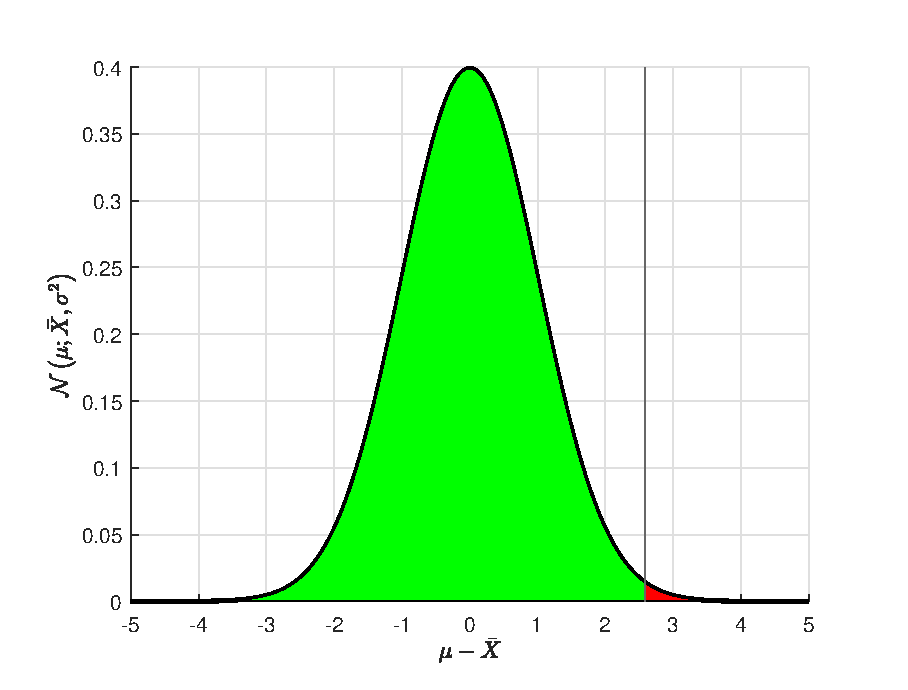
\includegraphics[width=250pt]{chapters/part-2/figures/hypothesis_normal_mean.eps}
	\caption{Distribution of $\mu$ as a function of $\mu^*$ and $\sigma^2$.} \label{ch:hypothesis_normal_mean}
\end{figure}

Draw a vertical bar at $\mu-\mu^*=C\textprime$ in Fig. \ref{ch:hypothesis_normal_mean} so that the area of the red zone equals to $\alpha$ and green zone $1-\alpha$. From \eqref{eq:intervalci},
\begin{eqnarray}
	C\textprime &=& \dfrac{u_\alpha}{\sqrt{m}}\sigma \nonumber
\end{eqnarray}
where $u_\alpha$ is a gain parameter determined by $\alpha$ as follows.
\begin{eqnarray}
	\textup{erf}\left(\dfrac{u_\alpha}{\sqrt{2}}\right) &=& 1-2\alpha \nonumber
\end{eqnarray}
For example, if $\alpha = 0.005$, $u_\alpha=2.58$. 

Consider a hypothesis test method where
\begin{eqnarray}
	\Phi : \left\{\begin{array}{cc}
		\textup{fail to reject~} H_0 & \mu_0 - \mu^* \leq C\textprime \\
		\textup{reject~} H_0 & \mu_0 - \mu^* > C\textprime
	\end{array}\right. \label{eq:hypotest_normal_2}
\end{eqnarray}
The hypothesis test \eqref{eq:hypotest_normal_2} can be interpreted as follows. From the empirical samples, $\mu$ is unlikely to be so large that it falls in the red zone in Fig. \ref{ch:hypothesis_normal_mean}. If the criterion $\mu_0$ is in the red zone, it is unlikely that $H_0: \mu > \mu_0$ is true. Therefore, the samples would reject $H_0$. On the other hand, if the criterion $\mu_0$ stays in the green zone, the samples fail to reject $H_0: \mu > \mu_0$ because it is fairly probable. 

For the above hypothesis test, the probability of $H_0$ being true while rejected equals to the area of the red zone which is $\alpha$. This hypothesis test meets the significance level of $\alpha$. 

Comparing \eqref{eq:hypotest_normal_1} and \eqref{eq:hypotest_normal_2} gives
\begin{eqnarray}
	C = \mu_0 - C\textprime = \mu_0 - \dfrac{u_\alpha}{\sqrt{m}}\sigma \nonumber
\end{eqnarray}
and \eqref{eq:hypotest_normal_1} becomes
\begin{eqnarray}
	\Phi : \left\{\begin{array}{cc}
		\textup{fail to reject~} H_0 & \mu^* \geq \mu_0 - \dfrac{u_\alpha}{\sqrt{m}}\sigma \\
		\textup{reject~} H_0 & \mu^* < \mu_0 - \dfrac{u_\alpha}{\sqrt{m}}\sigma
	\end{array}\right. \nonumber
\end{eqnarray}
which is a hypothesis test of the mean of a normal distribution at significance level of $\alpha$.

Consider $H_0$: $\mu = \mu_0$ and  $H_1$: $\mu \neq \mu_0$. The idea is similar except that there would have been two red zones in Fig. \ref{ch:hypothesis_normal_mean} at both tails. The hypothesis test is given by
\begin{eqnarray}
	\Phi : \left\{\begin{array}{cc}
		\textup{fail to reject~} H_0 & \mu_0 - \dfrac{u_\alpha}{\sqrt{m}}\sigma \leq \mu^* \leq  \mu_0 + \dfrac{u_\alpha}{\sqrt{m}}\sigma \\
		\textup{reject~} H_0 & \textup{otherwise}
	\end{array}\right. \nonumber
\end{eqnarray}
where notice that 
\begin{eqnarray}
	\textup{erf}\left(\dfrac{u_\alpha}{\sqrt{2}}\right) &=& 1-\alpha \nonumber
\end{eqnarray}
the $1-\alpha$ is used instead of $1-2\alpha$ on the right side of the above equation because the red zones are at both tails.

\subsection{The Variance of a Normal Distribution}

Variance is important in quality control. Let $X_i$ be $m$ samples taken from $\mathcal{N}(\mu, \sigma^2)$. The variance $\sigma^2$ is unknown. The objective is to use the samples to reject the following three types of null hypothesis
\begin{itemize}
	\item $H_0$: $\sigma^2 \geq \sigma_0^2$; $H_1$: $\sigma^2 < \sigma_0^2$
	\item $H_0$: $\sigma^2 \leq \sigma_0^2$; $H_1$: $\sigma^2 > \sigma_0^2$
	\item $H_0$: $\sigma^2 = \sigma_0^2$; $H_1$: $\sigma^2 \neq \sigma_0^2$
\end{itemize}
where $\sigma_0^2$ is the benchmark.

\subsection{The Comparison of Means of Two Normal Distribution}

The evaluation of the difference of two parameters is useful. It is widely used to compare the quality of two products. When the two parameters are described by normal distributions, the problem can be formulated as the comparison of the means of two normal distributions.

Let $X_i$ be $m$ samples taken from $\mathcal{N}(\mu_x, \sigma_x^2)$, and $Y_i$, $n$ samples from $\mathcal{N}(\mu_y, \sigma_y^2)$. The means $\mu_x$ and $\mu_y$ are unknown. The objective is to use the samples to reject the following null hypothesis
\begin{enumerate}
	\item $H_0$: $\mu_x - \mu_y \geq \mu_0$; $H_1$: $\mu_x - \mu_y < \mu^*$
	\item $H_0$: $\mu_x = \mu_y$; $H_1$: $\mu_x \neq \mu_y$
\end{enumerate} 
where $\mu_0$ is a given constant.

\subsection{Exponential Distribution}

As introduced earlier in Section \ref{sec:exponential_distribution}, exponential distribution can be used to model the duration of time between two independent events. It is useful to model the lifespan of an equipment, or the operating hour between its two consecutive independent and random failures.

Let $X_i$ be $m$ samples taken from \eqref{eq:exponential_pdf}. In practice, it can be $m$ sample products' lifespan. The expectation of \eqref{eq:exponential_pdf} is $\dfrac{1}{\lambda}$. The objective is to use the samples to estimate $\lambda$ and reject the following null hypothesis.
\begin{enumerate}
	\item $H_0$: $\lambda \geq \lambda_0$; $H_1$: $\lambda < \lambda_0$
	\item $H_0$: $\lambda \leq \lambda_0$; $H_1$: $\lambda > \lambda_0$
	\item $H_0$: $\lambda = \lambda_0$; $H_1$: $\lambda \neq \lambda_0$
\end{enumerate}
where $\lambda_0$ is a given constant.

\subsection{Binomial Distribution}

Let $X_i$ be $m$ samples taken from binomial distribution $\mathcal{B}(n,p)$, where $p$ is the probability of the Bernoulli trail, and $n$ be the number of trails repeated in the binomial test. The objective is to use the samples to reject the following null hypothesis.
\begin{enumerate}
	\item $H_0$: $p \geq p_0$; $H_1$: $p < p_0$
	\item $H_0$: $p \leq p_0$; $H_1$: $p > p_0$
	\item $H_0$: $p = p_0$; $H_1$: $p \neq p_0$
\end{enumerate}
where $p_0$ is a given constant.

\subsection{Poisson Distribution} 